\ifx\master\undefined
    \documentclass{scrartcl}
    \usepackage{authblk}
    \usepackage{amsmath}
    \usepackage{amssymb}
    \usepackage{amsthm}
    \usepackage{csquotes}
    \usepackage[british]{babel}
    \usepackage[
        giveninits,
        backend=biber,
        sorting=none,
        citestyle=numeric-comp,
        maxnames=10,
        style=vancouver,
    ]{biblatex}
    \usepackage{xr-hyper}
    \usepackage{hyperref}
    \usepackage{tabularx}
    \usepackage{booktabs}
    \usepackage{cleveref}
    \usepackage{fmtcount}
    \usepackage{environ}
    \usepackage{graphicx}
    \DeclareGraphicsExtensions{.pdf}

    \externaldocument{main}

    \usepackage[usenames]{xcolor}
    \definecolor{mpl0}{HTML}{1f77b4}

    \hypersetup{
        colorlinks=true,
        linkcolor=mpl0,
        citecolor=mpl0,
        urlcolor=mpl0,
    }

    \newcommand{\expit}{\sigma}
    \newcommand{\transpose}[1]{#1^\intercal}
    \DeclareMathOperator{\logit}{logit}
    \DeclareMathOperator{\logp}{log1p}
    \DeclareMathOperator{\logsumexp}{logsumexp}

    \newcommand{\abs}[1]{\left|#1\right|}
    \newcommand{\card}[1]{\left|#1\right|}
    \newcommand{\population}{N}
    \newcommand{\seeds}{U}
    \newcommand{\blauspace}{\mathbb{B}}
    \newcommand{\twocol}[1]{\multicolumn{2}{>{\hsize=\dimexpr2\hsize+3\tabcolsep+2\arrayrulewidth\relax}X}{#1}}

    \newcommand{\titlecaption}[2]{\caption[#1]{\emph{#1} #2}}
    \newtheorem{prop}{Proposition}
    \crefname{prop}{proposition}{propositions}

    \addbibresource{main.bib}


    % Royal Society Interface Guidance
    % Word-count: 2,500 to 8,000 words including cover page, references, and acknowledgements

    \title{Supplementary material}
    %\author{Till Hoffmann}
    %\author{Nick S. Jones}
    %\affil{Department of Mathematics, Imperial College London}
    \author{}
    \date{}
    %Buzz words -- inference, universal social scale, segregation measures, social kernel
    \begin{document}

    \maketitle
\fi

\appendix
\numberwithin{equation}{section}
\numberwithin{figure}{section}
\numberwithin{table}{section}

\begin{refsection}

The code to reproduce the results and figures is available at \url{https://github.com/tillahoffmann/kernels}.

\section{Evaluation of the observed-data log-likelihood}

\subsection{Weighting to account for non-uniform inclusion probabilities}

Seeds are often not included in the survey uniformly at random, and weights are traditionally used to compensate for the potentially biased selection of respondents~\cite{Kish1992}. Including weights in Bayesian analyses is generally difficult~\cite{Gelman2007}, and, in principle, we should model the data collection process explicitly~\cite[chapter~8]{Gelman2013}. Unfortunately, modelling the data collection process is non-trivial, and we use a weighted pseudo-likelihood instead~\cite{Pfeffermann1996}. In particular, the observed-data log-likelihood from \cref{eq:observed-likelihood-final} becomes
\begin{multline}
    L = \sum_{(i,j):I_{ij} = 1} w_j\left\{A_{ij} + (1 - A_{ij})w_i\right\}
    \\\times\left\{A_{ij}\log\rho_{ij} + (1-A_{ij})\log(1-\rho_{ij})-\log\left[r(0)(1 - \rho_{ij}) + r(1)\rho_{ij}\right]\right\},\label{eq:survey-weighted-log-likelihood}
\end{multline}
where $w_j$ is the weight associated with seed $j$. We clip all weights exceeding the \ordinalnum{95} percentile of the empirical weight distribution and normalise them such that $\sum_{j\in\seeds}w_j=\card{\seeds}$. Censoring the weights, also known as Winsorisation, limits the variance induced by attributing variable importance to different observations at the expense of introducing a small bias~\cite{Kish1992}.

\subsection{Numerical stability\label{app:numeric-stability}}

The evaluation of the observed-data log-likelihood may suffer from numerical instabilities, especially when the connectivity kernel $\rho(x, y, \theta)$ is small. We can mitigate such instabilities for logistic connectiviy kernels, i.e.
\begin{align}
    \rho(x,y,\theta)&=\expit(\transpose{\theta}f(x,y)),\\
    \text{where }\expit(\xi)&=\frac{1}{1+\exp(-\xi)}
\end{align}
is the logistic function. In particular, note that $1 - \expit(\xi) = \expit(-\xi)$ and $\log\expit(\xi)=-\logp\left[\exp(-\xi)\right]$, where $\logp(\xi)=\log(1 + \xi)$ is a numerically stable implementation---even for $\abs{\xi}\ll 1$. Substituting into \cref{eq:observed-likelihood-final} yields
\begin{multline}
    \log P(A|f,\theta,I=1)= -\sum_{(i,j):I_{ij}=1} A_{ij}\logp\exp\left(-\transpose{\theta}f_{ij}\right)+\left(1-A_{ij}\right)\logp\exp\left(\transpose{\theta}f_{ij}\right) \\
    + \logsumexp\left[\log r(0) - \logp\exp\left(\transpose{\theta}f_{ij}\right) + ,\log r(1)-\logp\exp\left(-\transpose{\theta}f_{ij}\right)\right],
\end{multline}
where $\logsumexp(x_1, \ldots, x_k)=\log\sum_{i=1}^k\exp(x_k)$ is a numerically stable implementation.

\section{Validation of inference methodology using synthetic ego network data\label{app:inference-validation}}

\begin{figure}
    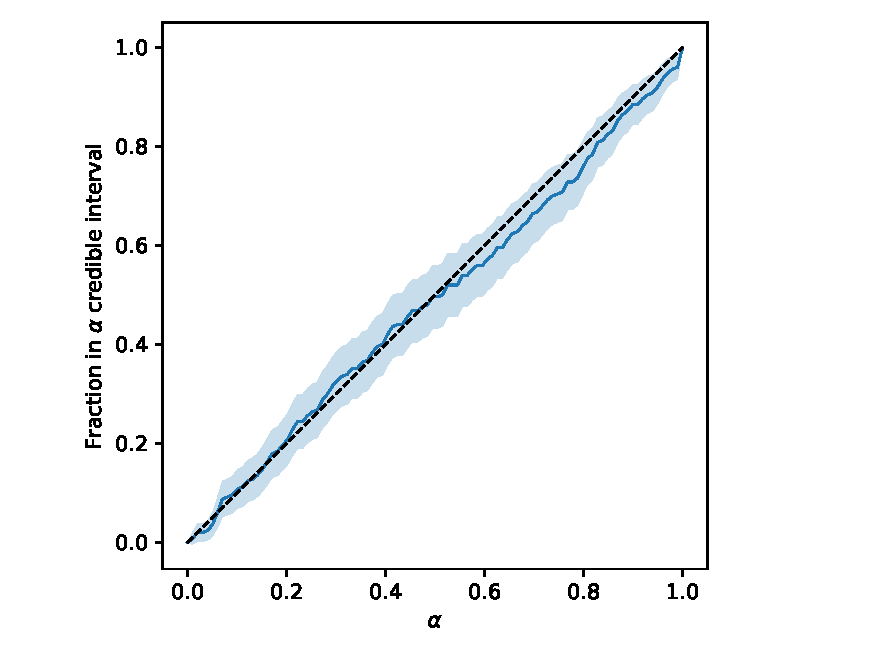
\includegraphics{credible-coverage}
    \titlecaption{A coverage analysis of posterior credible intervals validates the inference methodology.}{The blue line shows the fraction of inferences for which the true parameter values are contained in the $\alpha$-credible interval of a Laplace approximation of the posterior. The shaded region corresponds to two standard deviations of the mean across 250 simulations.\label{fig:credible-coverage}}
\end{figure}

To test the inference methodology, we conduct a coverage analysis of posterior credible intervals in three steps: fist, we generate 250 synthetic ego network datasets with known kernel parameter values. Second, we infer the parameter posterior distribution. Third, we evaluate the proportion $\lambda(\alpha)$ of true parameter values contained in the $\alpha$-credible interval across multiple synthetic datasets. We expect the true parameter values to be contained in the $\alpha$-credible interval for a proportion $\alpha$ of the synthetic datasets~\cite[section~10.7]{Gelman2013}, i.e.\ $\lambda(\alpha)\approx\alpha$.

In the first step, we draw the positions $x$ of $n=2,000$ nodes uniformly at random from the unit square, and we connect nodes to one another according to a logistic connectivity kernel with features
\begin{equation*}
    f(x_i, x_j) = \left(1, \frac{3 \left[\abs{x_{i1}-x_{j1}} - \frac{1}{3}\right]}{\sqrt{2}}, \frac{3 \left[\abs{x_{i2}-x_{j2}} - \frac{1}{3}\right]}{\sqrt{2}}\right),
\end{equation*}
where the first feature represents the bias, and the last two features capture distance in Blau space. The features were chosen to be standardised in the same fashion as described in \cref{sec:survey-gss}, i.e.\ to have zero mean and a standard deviation of $0.5$~\cite{Gelman2008a}. The corresponding parameter values $\theta$ are drawn from a normal distribution with unit variance and expectation
\begin{equation*}
    \left\langle \theta\right\rangle = \left(-7, 0, 0\right).
\end{equation*}
The expectation $\langle\theta\rangle$ was chosen such that it gives rise to a typical degree of $2,000 \times \expit(-7)\approx 1.8$, similar to the real-world datasets considered in \cref{sec:application}. We select $s=100$ respondents as egos and include all their alters as positive examples. We sample three times as many negative examples by selecting distinct pairs of respondents. If the number of respondents is not sufficient to draw the desired number of distinct control pairs, we use all $\frac{s(s-1)}{2}$ possible distinct pairs of respondents as negative examples.

In the second step, we maximise the log-posterior using a gradient ascent algorithm to obtain the MAP estimate $\theta$ and consider the Laplace approximation of the posterior~\cite[section~4.4]{Bishop2007}, i.e.\ a multivariate normal approximation in the vicinity of the MAP estimate. We evaluate the Hessian $H$ of the negative log-posterior at the MAP estimate to obtain the precision matrix of the Laplace approximation. We do not draw samples from the posterior because the Laplace approximation is computationally more convenient.

In the last step, we consider the quantity
\begin{equation}
   \chi^2 = \transpose{\left(\theta-\hat\theta\right)}H\left(\theta-\hat\theta\right)\label{eq:survey-chi2-statistic}
\end{equation}
which we expect to follow a $\chi^2$ distribution with three degrees of freedom~\cite{Slotani1964}. We calculate the statistic in \cref{eq:survey-chi2-statistic} for each simulation and consider the empirical probability that $\chi^2$ does not exceed the expected quantiles of the $\chi^2$-distribution, as shown in \cref{fig:credible-coverage}. As expected, the $\alpha$-credible interval contains the true parameter values for a fraction $\alpha$ of inferences, validating the inference methodology.

\section{Coding of demographic attributes and feature maps\label{app:coding-and-features}}

In the BHPS and USS, distance was coded as an ordinal variable: less than one mile, less than five miles, less than fifty miles, and more than fifty miles. We rely on having complete information about seeds to evaluate the control features in \cref{eq:logistic-kernel}. But data on the residential location of seeds is not made available to protect their privacy. Fortunately, we can sample the home locations of respondents\footnote{Sampling home locations cannot reproduce any correlation between home location and other demographic attributes.} using population estimates and the geographic boundaries of lower layer super output areas (LSOAs). LSOAs are census reporting areas and have a few thousand inhabitants each~\cite{Lsoas}. We approximate the distribution of distances between residents of the UK using rejection sampling: first, choose a LSOA with probability proportional to the number of residents. Second, choose one of the polygons associated with the LSOA with probability proportional to the area of the polygon (LSOAs are not necessarily contiguous). Third, sample points uniformly inside the bounding box of the polygon until a point inside the polygon is sampled. The last two steps assume uniform population densities within each LSOA, which is unlikely to be problematic as they are small areas. Having sampled the residential location of two respondents, we calculate the distance between respondents and cast to the same ordinal scale as reported for nominees. The USS furthermore distinguishes between friends living more than fifty miles apart but within the UK and friends outside the UK. We discard the latter (2.6\% and 2.1\% of all friends in waves C and F of the USS) because it is difficult to define an appropriate control population. For the BHPS, we implicitly assume that all friends are resident in the UK.

In the USS, respondents could identify with mixed ethnicities, and we coded such responses as a mixed membership. For example, a respondent who indicated ``mixed Asian and White'' would belong to both White and Asian ethnicities. To quantify how different two people are in terms of ethnicity, we define the feature map
\begin{equation*}
    f_\text{ethnicity}(x_i, x_j) = \frac{1}{2} \sum_{l\in E}\abs{x_{il}-x_{jl}},
\end{equation*}
where $E$ is the set of attributes encoding ethnic identity, and ethnicity memberships are normalised such that $\sum_{l\in E}x_{jl}=1$ for all $j$. For example, $f_\text{ethnicity}(x_i, x_j)=1$ for two people $i$ and $j$ one of which identifies as white and the other as black. For a person $i$ identifying as black and another person $j$ identifying as mixed black and Asian, $f_\text{ethnicity}(x_i, x_j)=0.5$.

\begin{table}
    \begin{tabularx}{\columnwidth}{lXXc}
        \toprule % =================================================================================
        Variable & Seed coding & Nominee coding & $f(x, y)$ \\
        \midrule % ---------------------------------------------------------------------------------
        Bias term &\twocol{\dotfill}& $1$\\
        Age & \twocol{Age in years\dotfill} & $\left|x-y\right|$\\
        Sex & \twocol{(a)~Male, (b)~Female\dotfill} & $x\neq y$\\
        Ethnicity & (a)~\{Asian Indian, Chinese, Filipino, Japanese, Korean, Vietnamese, Other Asian\} (b)~Black, (c)~Hispanic, (d)~White, (e)~\{American Indian or Alaska Native, Native Hawaiian, Guamanian or Chamorro, Samoan, Other Pacific Islander, Other\}& (a)~Asian, (b)~Black, (c)~Hispanic, (d)~White, (e)~Other & $x \neq y$\\
        Religion & (a)~Protestant, (b)~Catholic, (c)~Jewish, (d)~None, (e)~\{Other, Buddhism, Hinduism, Islam, Orthodox, Christian, Native American, Nondenominational\} & (a)~Protestant, (b)~Catholic, (c)~Jewish, (d)~None, (e)~Other & $x\neq y$ \\
        Education & (1)~1--6 years, (2)~7--12 years without high school diploma, (3) exactly 12 years with high school diploma, (4) $>12$ years without degree, (5)~Associate degree, (6)~Bachelor's degree, (7)~Professional or graduate degree & (1)~1--6 years, (2)~7--12 years, (3)~High school graduate, (4)~Some college, (5)~Associate degree, (6)~Bachelor's degree, (7)~Professional or graduate degree & $\left|x-y\right|$\\
        \bottomrule % ==============================================================================
    \end{tabularx}
    \titlecaption{Coding of the demographic variables for the General Social Survey together with the feature maps for each variable.}{Seeds were provided with 16 options to choose from for their own ethnicity but only five options for their nominees. We attempt to unify the educational coding by combining the number of years of education and formal qualifications of the seeds to approximate the coding of nominees. The bias term in the first row of the table controls the overall edge density.\label{tbl:survey-gss-coding}}
\end{table}

\begin{table}
    \begin{tabularx}{\columnwidth}{lrrrr}
        \toprule % =================================================================================
        Dataset & Egos & Dropped egos & Alters & Dropped alters \\
        \midrule % ------------------------------------------------------------------------------
        GSS '04 & 2,774 & 38 (1.4\%) & 863 & 158 (15.5\%)\\
        ALP '09 & 2,472 & 0 (0.0\%) & 2,481 & 315 (11.3\%)\\
        BHPS '92 & 9,105 & 1 (\textless 0.1\%) & 18,219 & 506 (2.7\%)\\
        BHPS '94 & 8,728 & 5 (0.1\%) & 17,328 & 469 (2.6\%)\\
        BHPS '98 & 8,584 & 5 (0.1\%) & 16,949 & 565 (3.2\%)\\
        BHPS '00 & 8,281 & 2 (\textless 0.1\%) & 16,255 & 432 (2.6\%)\\
        BHPS '02 & 7,971 & 0 (0.0\%) & 15,716 & 502 (3.1\%)\\
        BHPS '04 & 7,609 & 0 (0.0\%) & 14,971 & 502 (3.2\%)\\
        BHPS '06 & 7,459 & 0 (0.0\%) & 14,558 & 331 (2.2\%)\\
        USS '11 & 36,526 & 199 (0.5\%) & 74,141 & 461 (0.6\%)\\
        USS '14 & 29,082 & 319 (1.1\%) & 61,892 & 611 (1.0\%)\\
        \bottomrule % ==============================================================================
    \end{tabularx}
    \titlecaption{Number of retained seeds and nominees for each dataset together with the number of individuals who have been excluded from the analysis because one or more of their demographic attributes were missing.}{Individuals excluded for other reasons, e.g.\ due to being a relative or under the age of 18, are not listed.\label{tbl:survey-sample-size}}
\end{table}

\begin{table}
    \begin{tabularx}{\columnwidth}{lXXc}
        \toprule % =================================================================================
        Variable & Seed coding & Nominee coding & $f(x, y)$ \\
        \midrule % ---------------------------------------------------------------------------------
        Bias term &\twocol{\dotfill}& $1$\\
        Age & Age in years recoded to match the nominee coding & Age brackets in years: (1)~0--20, (2)~21--35, (3)~36--50, (4)~51--65, (5)~66--80, (6)~$>80$ & $\left|x-y\right|$\\
        Sex & \twocol{(a)~Male, (b)~Female\dotfill} & $x\neq y$\\
        Ethnicity & \twocol{(a)~White or Caucasian, (b)~Black or African American, (c)~American Indian or Alaska Native, (d)~Asian or Pacific Islander, (e)~Hispanic (see below) (f)~Other} & $x \neq y$\\
        Hispanic & \twocol{(a)~Yes, (b)~No; ethnicity is coded as ``Hispanic'' if response is affirmative.\dotfill} & \\
        Education & \twocol{The seed coding is more refined but can be reduced to the nominee coding: (1)~Less than \ordinalnum{9} grade, (2)~\ordinalnum{9}--\ordinalnum{12} grade without diploma, (3)~High school graduate, (4)~Some college, (5)~Associate degree, (6)~Bachelor's degree, (7)~Master's degree, (8)~Professional degree or doctorate\dotfill} & $\left|x-y\right|$\\
        State & \twocol{One of 52 states and Washington DC and Puerto Rico\dotfill} & $x \neq y$\\
        \bottomrule % ==============================================================================
    \end{tabularx}
    \titlecaption{Coding of the demographic variables for the American Life Panel together with the feature maps for each variable.}{We aggregate the ages and educational attainments of seeds to match the coarser coding of nominees, as shown in \cref{tbl:survey-alp-coding}. The joint effect of ethnic differences and whether people identify as Hispanic is still unclear~\cite{Smith2017a}; for consistency with the GSS, we code the ethnicity of respondents as ``Hispanic'' if they consider themselves to be Hispanic or Latino irrespective of their reported ethnicity. In fact, 46\% of respondents who identified as Hispanic selected ``other'' as their ethnicity, compared with $<1\%$ for respondents who did not identify as Hispanic.\label{tbl:survey-alp-coding}}
\end{table}

\begin{table}
    \noindent\begin{minipage}{\columnwidth}
    \renewcommand*\footnoterule{}
    \begin{tabularx}{\columnwidth}{lXXc}
        \toprule % =================================================================================
        Variable & Seed coding & Nominee coding & $f(x, y)$ \\
        \midrule % ---------------------------------------------------------------------------------
        Bias term &\twocol{\dotfill}& $1$\\
        Age & \twocol{Age in years\dotfill} & $\left|x-y\right|$\\
        Sex & \twocol{(a)~Male, (b)~Female\dotfill} & $x\neq y$\\
        Occupation & (a)~\{Self-employed, employed, maternity leave, unpaid worker in family business\footnote{\label{ft:survey-only-usoc}Only available in Understanding Society.}\}, (b)~\{Unemployed, disabled\}, (c)~\{Full-time student, government training scheme\}, (d)~Family care, (e)~Retired & (a)~\{Full-time employed, part-time employed\}, (b)~Unemployed, (c)~Full-time education, (d)~Full-time housework, (e)~Retired & $x \neq y$\\
        Distance & Only applicable to the seed-nominee pair & (1)~$<1~\mathrm{mile}$, (2)~$<5~\mathrm{miles}$, (3)~$<50~\mathrm{miles}$, (4)~$\geq50~\mathrm{miles}$ but still in the UK &\footnote{We use the ordinal distance reported in the survey as a regression feature and generate control features using Monte Carlo simulation, as discussed in \cref{app:coding-and-features}.}\\
        Ethnicity\footref{ft:survey-only-usoc} & \twocol{Independent binary choices: White, Asian, Black, Other\dotfill} &\footnote{See \cref{app:coding-and-features} for a detailed description of the feature map.}\\
        \bottomrule % ==============================================================================
    \end{tabularx}
    \end{minipage}
    \titlecaption{Coding of the demographic variables for the British Household Panel Survey and Understanding Society together with the feature maps for each variable.}{Sex and age have identical coding for seeds and nominees. We aggregate the detailed occupational coding of seeds to match the coding of nominees. In particular, we code women on maternity leave as employed because their occupational status is only temporary, and we code disabled individuals as ``not employed'' because they are unlikely to have the same social opportunities as people in employment.\label{tbl:survey-usoc-coding}}
\end{table}

\printbibliography

\end{refsection}

\ifx\master\undefined
\end{document}
\fi
